\section{Robot design}
Designet af robotten for dette projekt er yderst vigtigt; det er grundstenen i projektet, og uden en velfungerende robot (og specifikt kontrol af denne), vil det blive yderst svært at løse problemstillingen for projektet tilfredsstillende.
At navigere et ukendt areal med en kendt position kræver præcis kontrol af enhver bevægelse, hvorfor dette afsnit fokuserer på hvordan vi er kommet frem til designet af den endelige robot samt hvilke særlige problemstillinger der ligger til grund for designet.

\subsection{Design overvejelser}
Designet af robotten har været en del af læringsprocessen for hvordan man bygger en robot af \lego NXT komponenterne, hvorfor design processen kan ses som en iterativ process, hvor designet er blevet radikalt ændret for hver iteration indtil et tilfredsstillende resultat er opnået.

\subsubsection{Første design}
Test test 

\subsubsection{Andet design}

\subsubsection{Tredje design}


\begin{figure}
\centering
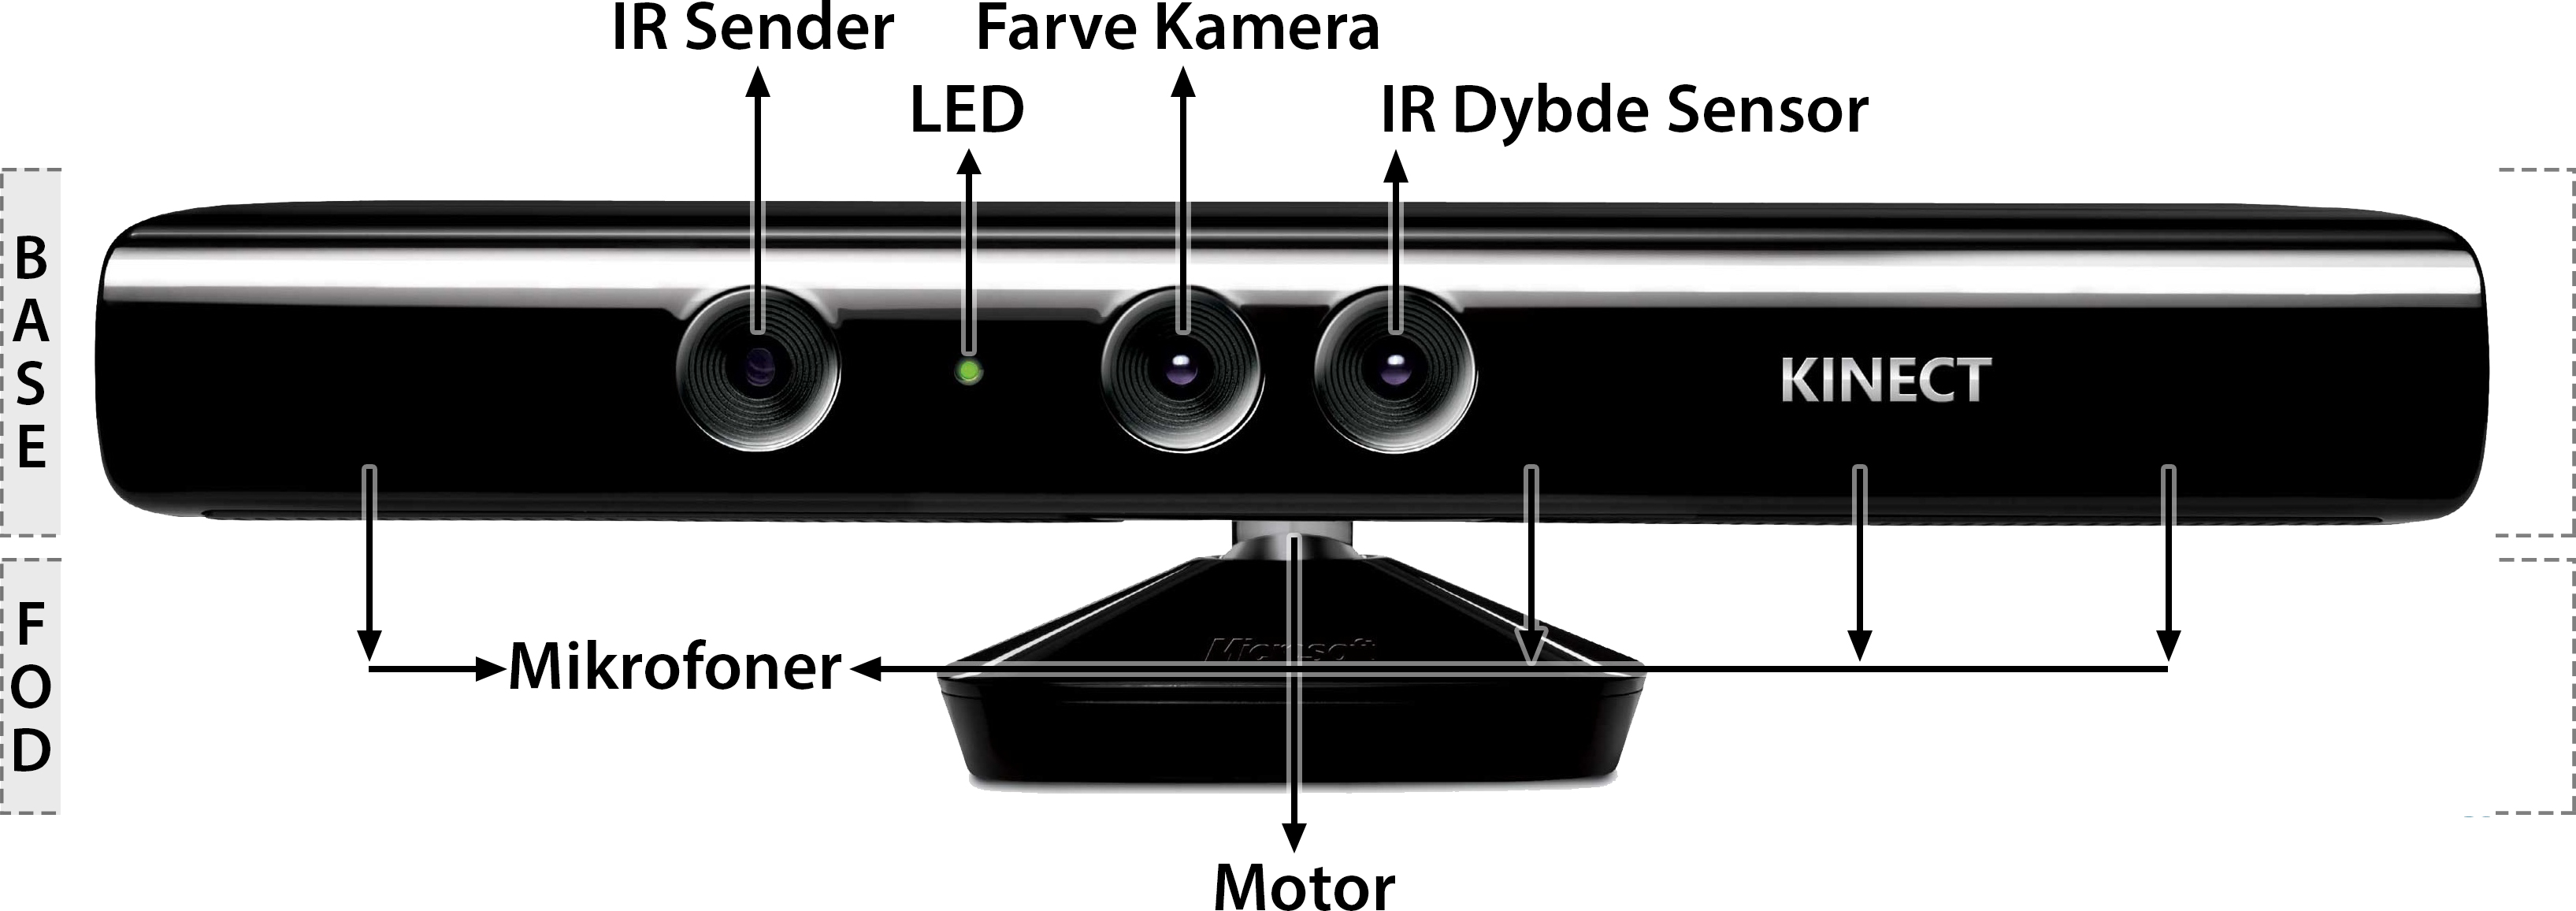
\includegraphics[width=0.5\textwidth]{kinect/kinect}
\caption{Endelige design af vores robot.}
\label{robot:opbygning}
\end{figure}

\subsection{Komponenters placering}


\subsubsection{Basen}

\subsubsection{Fremdrift}
- valg af hjul og fremdrift
- grund til gearing

\subsubsection{Sensorer}
- sensorens placering og mobilitet


\section{Gearing}
- grund til valg af gearings tal